\section{Zielsetzung}
In diesem Versuch werden Magnetfelder gemessen, welche durch unterschiedliche Spulenanordnungen erzeugt werden.
Der letzte Teil des Versuchs befasst sich zudem mit der durch eine Ringspule erzeugten Hysteresekurve.

\section{Theorie}
Den Raum um einen Magneten bezeichnet man als Magnetfeld, welches eine Vektorgröße ist, der eine magnetische Feldstärke $\vec{H}$ zugeordnet wird. Darstellen lässt sich
das Feld mithilfe von geschlossenen Feldlinien. 
Wird die Feldstärke $\vec{H}$ mit der materialspezifischen magnetischen Permeabilität $\mu$ verbunden, so ergibt sich die magnetische Flussdichte $\vec{B}$
\begin{equation}
\label{eqn:bmuh}
\vec{B} = \mu \cdot \vec{H}
\end{equation}
mit
\begin{equation*}
\mu = \mu_0 \cdot \mu_{\text{r}},
\end{equation*}
wobei $\mu_0$ die Vakuum-Permeabilität ist und $\mu_{\text{r}}$ die relative Permeabilität in Materie.

Auch stromdurchflossene Leiter sind aufgrund des Ladungsstroms von Magnetfeldern umgeben. Dabei verlaufen die Feldlinien senkrecht zum Stromfluss in konzentrischen 
Kreisen um den Leiter. Die Magnetfeldstärke $\vec{H}$ im Abstand $r$ von einem Leiter, welcher vom Strom $I$ durchflossen wird, kann mit dem Biot-Savart-Gesetz und der 
Vakuum-Permeabilität $\mu_0$ = $4\pi \cdot 10^{-7}$ berechnet 
werden:
\begin{equation*}
\symup{d}\vec{B} = \frac{\mu_0 I}{4 \pi} \frac{\symup{d}\vec{s} \times \vec{r}}{r^3}.
\end{equation*}
Das Biot-Savart-Gesetz lässt sich ebenso auf stromdurchflossene Spulen anwenden. Die magnetische Flussdichte in der Mitte der Spule ist dann
\begin{equation*}
\vec{B}(x) = \frac{\mu_0 I}{2} \frac{R^2}{(R^2 + x^2)^{\frac{3}{2}}} \cdot \hat{x}.
\end{equation*}
Bei einer Spule mit $n$ Windungen erhöht sich der magnetische Fluss um Faktor $n$.

Bei einer langen Spule ist Magnetfeld in der Mitte der Spule homogen, das heißt konstant, da die Feldlinien dort parallel verlaufen. An den Enden der Spulen sowie 
im Außenbereich ist das Magnetfeld inhomogen, weil sich die Magnetfeldlinien ausbreiten und die Spule umschließen. Das homogene Feld im Inneren kann mit 
\begin{equation}
\label{eqn:formel1}
B = \mu_{\text{r}}\mu_0 \frac{n}{l}I
\end{equation}
berechnet werden, wobei $l$ die Spulenlänge ist, $n$ die Windungszahl und $I$ der Strom, der durch die Spule fließt.

Wird die lange Spule zu einem Ring gebogen, so verschwindet das Feld außen und es bleibt nur das homogene Magnetfeld innerhalb des Torus. Dann ergibt sich mit
$l = 2\pi r_{\text{T}}$ das Magnetfeld
\begin{equation}
\label{eqn:formel2}
B = \mu_{\text{r}} \mu_0 \frac{n}{2\pi r_{\text{T}}} I.
\end{equation}

Um ein homogenes Magnetfeld zu erzeugen, kann ein Helmholtz-Spulenpaar verwendet werden, das aus zwei Kreispulen im Abstand des Spulenradius R besteht, die 
gleichsinnig vom Strom $I$ durchflossen werden. Die Felder der beiden Spulen, die mit dem Biot-Savart-Gesetz berechnet werden, überlagern sich und können nach dem 
Superpositionsprinzip addiert werden:
\begin{equation*}
B(0) = B_1(x) + B_1(-x) = \frac{\mu_0 I R^2}{(R^2 + x^2)^{\frac{3}{2}}}.
\end{equation*}

In der Physik sind verschiedene Arten von magnetischen Materialien bekannt. Ein Beispiel sind Ferromagneten, zu denen Eisen gehört. Diese Materialien haben ein
eigenes dauerhaftes magnetisches Moment, welches sich jeweils in den sogenannten Weiß'schen Bezirken im Körper parallel zueinander ausrichten. Mittels eines äußeren
Magnetfeldes können die Bezirke vergrößert werden, was die magnetische Energie des Körpers erhöht.

Ferromagnetische Materialien besitzen eine hohe relative Permeabilität, was dazu führt, dass die Gleichung \eqref{eqn:bmuh} aufgrund der Nichtlinearität nicht 
anwendbar ist. Dargestellen lässt sich dies mit einer Hysteresekurve, wie in Abbildung \ref{fig:hysteresekurve} zu sehen ist.
\begin{figure}[h!]
	\centering
	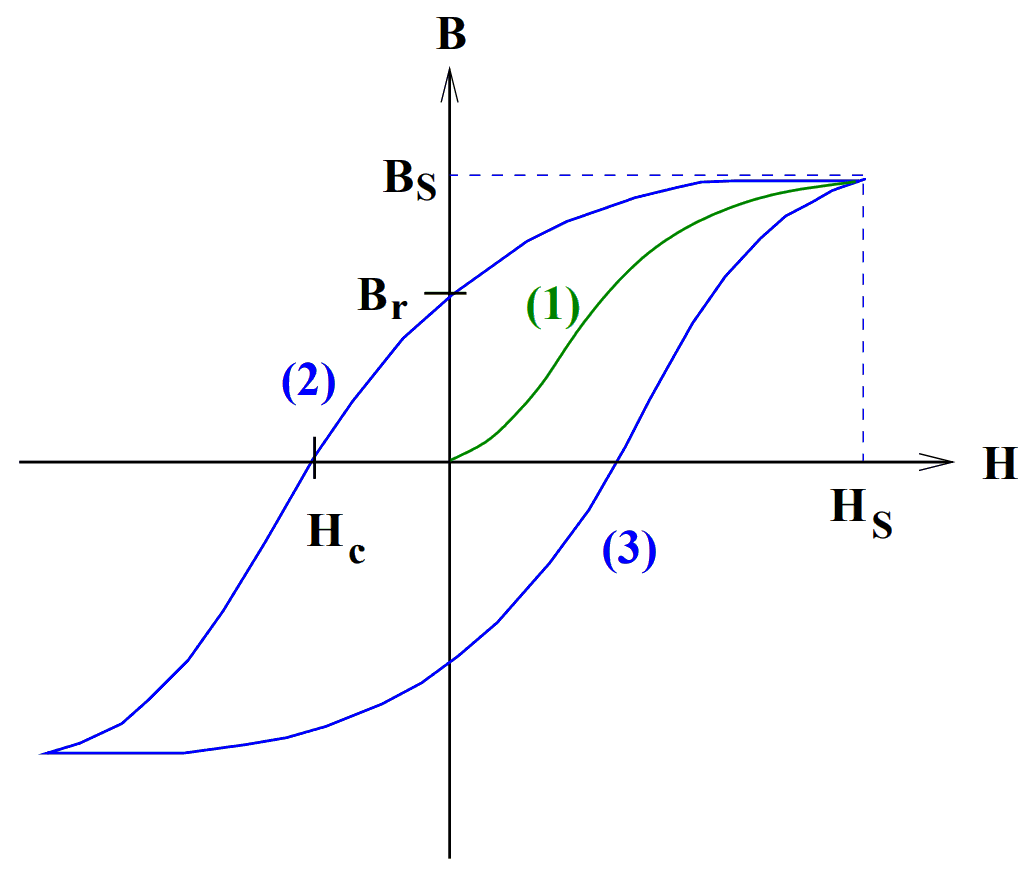
\includegraphics[width=0.6\linewidth]{../../Hysteresekurve}
	\caption{Schematische Darstellung der Hysteresekurve, \cite[3]{anleitung308}.}
	\label{fig:hysteresekurve}
\end{figure}
Zur Erzeugung der Hysteresekurve wird der Ferromagnet einem äußeren Magnetfeld ausgesetzt. Zunächst ist das äußere Feld Null und wird dann erhöht, sodass die 
Magnetisierung des Materials bis zu dem Sättigungswert $B_{\text{r}}$ steigt, was in (1), der Neukurve, zu sehen ist. Wird das äußere Feld verringert, so kehrt sich die 
Magnetisierung um und breitet sich mit stärkerem äußeren Feld über das ganze Material aus (2). Wenn das äußere Feld wieder Null beträgt ist allerdings zu beobachten, 
dass die Magnetisierung nicht wieder Null ist. Es bleibt also eine Remanenz, die mit einem Gegenfeld, der Koerzitivkraft, aufgehoben werden kann. Wird das Gegenfeld 
erhöht, so wird die Magnetisierung negativ, bis der Sättigungswert $-B_{\text{r}}$ erreicht wird. Durch erneute Umpolung
entsteht dann die restliche Hysteresekurve (3), die symmetrisch zur ersten Kurve verläuft. Die Form dieser Kurve ist materialabhängig.

Mithilfe eines ferromagnetisches Kerns kann der magnetische Fluss einer Spule erhöht werden:
\begin{equation*}
\vec{B} = \mu_0 (\vec{H} + \vec{M}).
\end{equation*}
Zu sehen ist, dass diese Erhöhung von der Magnetisierung des Materials abhängt.  Mit $\vec{H} = \vec{H_0} + \vec{H_{\text{R}}}$ werden bei einer einfachen Spule die
Randeffekte berücksichtigt, bei Tori fallen diese Randeffekte weg.

In diesem Versuch werden zur Messung der Magnetfelder Hallsonden verwendet, welche ein Leiterplättchen besitzen, durch das ein Strom fließt. Das zu messende Magnetfeld
übt auf die bewegten Elektronen eine Lorentzkraft auf, durch die eine Ladungstrennung und dadurch eine Hallspannung ensteht. Diese Spannung wird direkt gemessen und ist ein
Maß für das Magnetfeld. 